\subsubsection*{Waypoint table}
Tabellen indeholder alle waypoints som brugeren har oprettet i systemet. Hvert waypoint i tabellen indeholder information om gps-koordinatet, højden og om der skal tages et billede på den givet lokation eller ej.
\vspace{-5pt}
\begin{figure}[H]
	\centering
	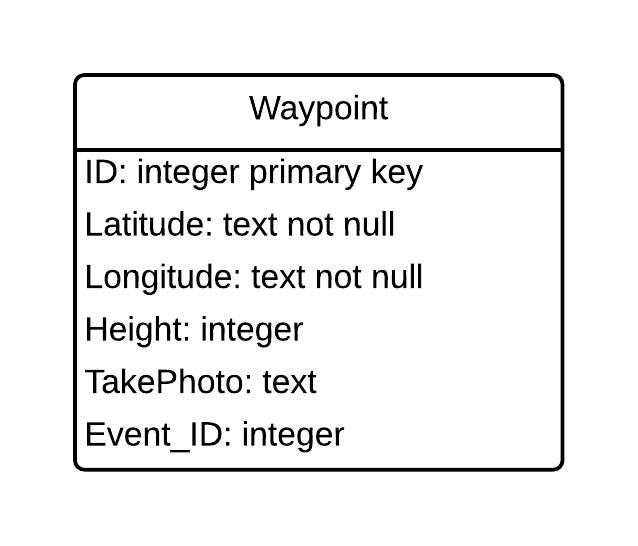
\includegraphics[width=0.5\textwidth]{Billeder/database/WaypointTable.png}
	\vspace{-5pt}
	\caption{Waypoint table}
	\label{fig:waypoint_table}
\end{figure}

\begin{table}[H]
\begin{tabular}{| p{3cm}| p{11.5cm}|}
\hline

Formål	 							& Holde data om waypoints i systemet.\\\hline
Forbindelser						& Tabellen har en foreing key til event tabllen.\\\hline
Attributter						& \begin{itemize}
												\item ID: Primary key.
												\item Latitude: Requried text felt. Max length: 100 char
												\item Longitude: Requried text felt. Max length: 100 char
												\item Height: integer
												\item Event ID: Relation til event tabellen: Foreingkey
											\end{itemize} \\\hline 
\end{tabular}
\caption{Waypoint table}
\label{tab:waypoint_table}
\end{table}